\chapter{Architettura Funzionale del Sistema Realizzato}
\section{Obiettivi dell'applicativo}
Lo scopo principale dell'applicativo sviluppato \`e quello di fornire un servizio per la visualizzazione delle immagini scattate dai diversi Rover inviati su Marte nel corso degli ultimi anni.\\
Queste immagini possono essere visualizzate sul proprio dispositivo mobile con sistema operativo Android o iOS, tramite una applicazione che pu\`o essere scaricata da un sito web online.

L'applicazione dovr\`a fornire una funzione di ricerca, tramite la quale si potranno ricercare immagini inserendo il nome di uno dei Rover oppure digitando la data solare in cui sono state scattate le immagini che si vogliono osservare. In particolare, i nomi dei Rover per i quali si potr\`a effettuare una ricerca sono: Curiosity,Spirit e Opportunity.
Tra una ricerca e l'altra verr\`a mostrata una schermata di ``loading" in modo da indicare all'utente che si sta eseguendo il ``fetching" delle immagini.

Oltre a poter ricercare le immagini secondo diversi parametri, l'applicazione dovr\`a anche fornire la possibilit\`a di nascondere alcune di queste in modo che non vengano visualizzate dall'utente in una ricerca futura.
Nonostante le immagini nascoste non vengano presentate all'utente quando effettua una ricerca, gli verr\`a sempre concessa la possibilit\`a di ripristinarle.

L'utente potrebbe non essere interessato ad un'intera categoria di immagini, quindi gli verr\`a fornita la possibilit\`a di nascondere tutte le foto relative ad una sua ricerca.

Ogni volta che verr\`a chiusa l'applicazione, le ultime immagini visualizzate dovranno essere memorizzata in modo persistente cos\`i che possano essere mostrate all'ultilizzatore quando riaprir\`a l'app.

Oltre a poter visualizzare le immagini in una lunga lista nell'Index Screen dell'applicazione, quest'ultima dovr\`a fornire anche la possibilit\`a di visualizzare i dettagli di ognuna di esse.

Al primo avvio l'utente dovr\`a essere ridirezionato verso una schermata di login o di registrazione a seconda che sia in possesso o meno delle credenziali di accesso.

\section{Requisiti dell'applicativo}
\subsection{Requisiti necessari per il funzionamento dell'applicativo}

L'applicazione necessita di una connessione ad Internet in modo da collegarsi
tramite il web ai server della Nasa e recuperare le immagini ricercate da ogni utente.

%Ogni utente la prima volta che accede all'applicazione o quando effettua il ``logout" da essa, deve inserire le proprie credenziali in modo da poter accedere all'Index Screen.\\
Le credenziali di ogni utente sono memorizzate in un database distribuito che memorizza i dati in documenti flessibili JSON-like. In particolare, per assicurare la sicurezza di ogni utilizzatore, le password di ognuno di essi vengono memorizzate
solo dopo essere state cifrate. In questo modo anche se qualcuno dovesse penetrare nel database non riuscirebbe ad accedere ai vari account.

Il database viene consultato attraverso un server locale che espone delle API all'applicativo per far s\`i che ogni utente possa eseguire la registrazione e il login.
Affinch\'e l'applicazione possa comunicare con il server locale, deve essere attiva un'applicazione Multipiattaforma chiamata Ngrok\footnote{Ngrok consente di aprire una connessione diretta verso le API sviluppate in Express e fornisce un URL tramite il quale il dispositivo mobile pu\`o usufruirne. In particolare, espone le porte su cui i server locali sono in ascolto ad Internet.}.


Per garantire l'efficienza dell'applicazione il numero di immagini recuperate, ad ogni richiesta GET ai server della Nasa, deve essere pari a 25. In questo modo si evita di sovraccaricare il client che deve elaborare le immagini e presentarle a schermo.

Di seguito si pu\`o osservare una rappresentazione grafica dell'interazione tra i vari sistemi:
\begin{figure}[h]
    \centering
    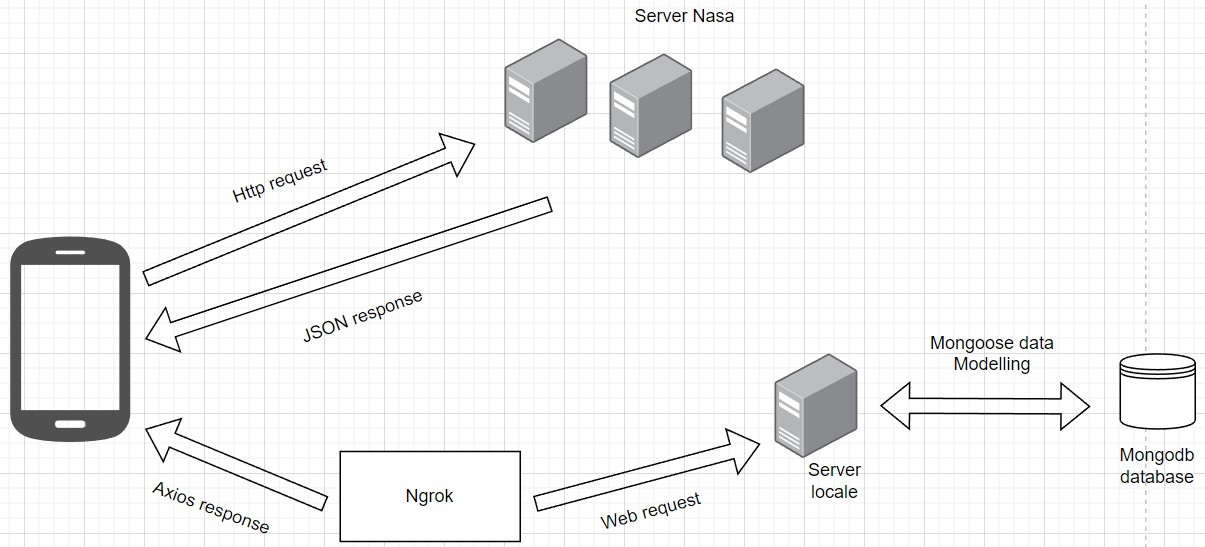
\includegraphics[width=13cm, height=7cm]{images/ModelloDiComunicazioneApplicazione.jpg}
    \caption[differenzeiteot]{}
    \label{fig:modellodicomunicazione}
\end{figure}
\subsection{Requisiti funzionali}

Ad ogni requisito viene associato un nome mnemonico, una breve descrizione e un codice di priorit\`a in modo tale da indicare quali requisiti devono essere implementati per primi e quindi definire una gerarchia di implementazione.
\begin{center}
    \begin{longtable}{ | l | p{7cm} | l | }
        \hline
        \textbf{Nome}      & \textbf{Descrizione }                                                                                                     & \textbf{Priorit\`a} \\ \hline
        Sign in            & L'utente deve poter accedere all'applicazione tramite le sue credenziali                                                  & Primario            \\ \hline
        Sign up            & L'utente deve potersi registrare tramite la propria e-mail e password in modo da poter accedere all'applicazione          & Primario            \\ \hline
        Search by name     & L'utente deve poter ricercare le immagini tramite il nome di uno dei tre possibili Rover: Spirit, Opportunity e Curiosity & Primario            \\ \hline
        Search by date     & L'utente deve poter ricercare le immagini che sono state scattate in una precisa data solare                              & Primario            \\ \hline
        Hide image         & L'utente deve poter nascondere le immagini che gli vengono presentate                                                     & Primario            \\ \hline
        Restore images     & L'utente deve poter ripristinare le immagini che ha nascosto                                                              & Secondario          \\ \hline
        Logout             & L'utente deve poter uscire dal proprio profilo                                                                            & Secondario          \\ \hline
        Hide all           & L'utente deve poter nascondere nascondere tutte le ommagini relative ad una sua ricerca                                   & Secondario          \\ \hline
        Privacy and Policy & L'utente deve poter conoscere quali condizioni e termini ha accettato scaricando l'applicazione                           & Secondario          \\ \hline
    \end{longtable}
\end{center}
\subsection{Requisiti non funzionali}
In questa sezione verranno descritti i principali requisiti non funzionali necessari per il buon funzionamento dell'applicazione.
\begin{center}
    \begin{longtable}{ | l | p{7cm} | }
        \hline
        \textbf{Nome}    & \textbf{Descrizione }                                                                                                       \\ \hline
        Prestazioni      & L'applicativo deve essere in grado di presentare le immagini entro 6 secondi dall'avvio della ricerca                       \\ \hline
        Portabilit\`a    & L'applicativo deve poter essere scaricabile sia su dispositivi iOS che Android                                              \\ \hline
        Manutenibilit\`a & L'applicativo deve essere strutturato seguendo un architettura modulare in modo da facilitare la fase di test e di modifica \\ \hline
    \end{longtable}
\end{center}

\section{Casi d'uso}

In questa sezione verranno illustrati i pricipali casi d'uso.%In ognuno di essi gli attori\footnote{L'attore \`e qualsiasi entit\`a che svolge un ruolo in un dato sistema. Questo potrebbe essere una persona, un'organizzazione o un sistema esterno. } sono gli end users e il server locale.
\subsection*{Caso d'uso U1: Sign in}
\begin{itemize}
    \item  \textbf{Use case overview:} l'applicazione deve consentire agli utenti la possibilit\`a di poter accedere al proprio account.
    \item \textbf{Actors:} end user, server locale.
    \item \textbf{Triggers:} si preme sul pulsante ``Sign in".
    \item \textbf{Pre-Condition:} l'utente non deve aver gi\`a effettuato l'accesso all'applicazione oppure si deve trovare nell'Index Screen dove pu\`o effettuare il logout.
    \item \textbf{Post-condition:} si verr\`a indirizzati nell'Index Screen dell'applicazione.
    \item \textbf{Main Flow:} \begin{enumerate}
              \item L'utente ha appena terminato di scaricare l'applicazione e la apre, ritrovandosi come prima schermata lo ``Splash screen". Una volta premuto il pulsante ``Explore" verr\`a reindirizzato sullo screen destinato al log in.
              \item Arrivato allo screen di log in l'utente inserir\`a la propria e-mail e password e premer\`a sul pulsante ``Sign in".
              \item Verr\`a inviata una richiesta al server locale che andr\`a a confrontare le credenziali inserite in precedenza con quelle presenti sul database per verificare che coincidano. In caso affermativo l'utente verr\`a indirizzato sull'Index Screen.

          \end{enumerate}
    \item \textbf{Alternative Flow:}\begin{enumerate}
              \item L'utente si trova nell'Index Screen e sta scorrendo tutta la lista di immagini a lui presentate. Una volta arrivato alla fine della lista premer\`a sul pulsante di ``logout".
              \item L'utente si ritrover\`a nello screen riservato al log in dove inserir\`a la propria mail e password e premer\`a sul pulsante ``Sign in".
              \item Verr\`a inviata una richiesta al server locale che andr\`a a confrontare le credenziali inserite in precedenza con quelle presenti sul database per verificare che coincidano. In caso affermativo l'utente verr\`a indirizzato sull'Index Screen.
          \end{enumerate}

    \item \textbf{Exception Flow:}\begin{enumerate}
              \item Una volta inserite le proprie credenziali verr\`a inviata una richiesta al server locale che andr\`a a confrontare quest'ultime con quelle presenti sul database.
              \item Le credenziali inserite dall'utente non sono corrette e gli viene presentato un messaggio di errore. \end{enumerate}
\end{itemize}
\subsection*{Caso d'uso U2: Sign up}
\begin{itemize}
    \item  \textbf{Use case overview:} l'applicazione deve consentire agli utenti la possibilit\`a di potersi registrare tramite la propria e-mail e password.
    \item \textbf{Actors:} end user, server locale.
    \item \textbf{Triggers:} si preme sul pulsante ``Sign up".
    \item \textbf{Pre-Condition:} l'utente non deve aver gi\`a effettuato l'accesso all'applicazione.
    \item \textbf{Post-condition:}si verr\`a indirizzati nell'Index Screen dell'applicazione.
    \item \textbf{Main Flow:} \begin{enumerate}
              \item L'utente ha appena terminato di scaricare l'applicazione e la apre, ritrovandosi come prima schermata lo ``Splash screen". Una volta premuto il pulsante "Explore" verr\`a reindirizzato sullo screen destinato al log in. Non avendo alcune credenziale valida l'utente dovr\`a premere sul pulsante "Sign up" in modo da essere reindirizzato nello schermo dedicato alla registrazione.
              \item Arrivato allo screen di registrazione l'utente inserir\`a la propria e-mail e password e premer\`a sul pulsante ``Sign up".
              \item Verr\`a inviata una richiesta al server locale che andr\`a a confrontare che l'e-mail inserita dall'utente non sia gi\`a presente nel database. In caso affermativo l'utente verr\`a indirizzato sull'Index Screen.

          \end{enumerate}

    \item \textbf{Exception Flow:}\begin{enumerate}
              \item Una volta inserite le proprie credenziali verr\`a inviata una richiesta al server locale che andr\`a a confrontare che l'e-mail inserita dall'utente non sia gi\`a presente nel database.
              \item Esiste gi\`a un utente registrato con quella e-mail, quindi il sistema restituisce un messaggio di errore. \end{enumerate}
\end{itemize}
\subsection*{Caso d'uso U3: Ricerca immagini tramite nome Rover}
\begin{itemize}
    \item  \textbf{Use case overview:} l'applicazione deve consentire agli utenti la possibilit\`a di ricercare le immagini in base al nome del Rover.
    \item \textbf{Actors:} End user, server Nasa.
    \item \textbf{Triggers:} si digita il nome di uno dei tre Rover nella Search Bar e si preme ``fatto" sulla propria tastiera.
    \item \textbf{Pre-Condition:} l'utente deve aver effettuato l'accesso oppure essere in possesso di un JSON Web Token.
    \item \textbf{Post-condition:} verranno presentate delle nuove immagini o una modale che informa l'utente che nessuna immagine \`e stata trovata.
    \item \textbf{Main Flow:} \begin{enumerate}
              \item L'utente si trova nella schermata principale e digita il nome del Rover che ha scattato le immagini richieste. Per avviare la ricerca si dovr\`e premere sul pulsante ``All".
              \item Viene effettuata una richiesta HTTP verso i server della Nasa i quali rispondono con un oggetto JSON che contiene tutte le foto che sono state trovate.
              \item Le immagini ottenute vengono inserite all'interno di una lista e vengono visualizzate a schermo.

          \end{enumerate}
    \item \textbf{Alternative Flow:}\begin{enumerate}
              \item L'utente si trova nella schermata principale e digita il nome del Rover che ha scattato le immagini le immagini richieste. Per avviare la ricerca si dovr\`e premere sul pulsante ``All".
              \item Viene effettuata una richiesta HTTP verso i server della Nasa i quali rispondono con un oggetto JSON che contiene tutte le foto che sono state trovate.
              \item Il nome del Rover inserito non \`e corretto. L'utente viene informato che non \`e stata trovata alcuna foto e gli viene presentata una lista di immagini vuota.

          \end{enumerate}
\end{itemize}
\subsection*{Caso d'uso U4: Ricerca immagini per data solare}
\begin{itemize}
    \item  \textbf{Use case overview:} l'applicazione deve consentire agli utenti la possibilit\`a di ricercare le immagini in base a una certa data solare.
    \item \textbf{Actors:} end user, server Nasa.
    \item \textbf{Triggers:} si preme sul pulsante ``Search by date".
    \item \textbf{Pre-Condition:} l'utente deve aver effettuato l'accesso oppure essere in possesso di un JSON Web Token.
    \item \textbf{Post-condition:} verranno presentate delle nuove immagini o una modale che informa l'utente che nessuna immagine \`e stata trovata.
    \item \textbf{Main Flow:} \begin{enumerate}
              \item L'utente si trova nell'Index Screen e preme il pulsante ``Data" in modo da spostarsi nello schermo dedicato alla ricerca per data solare. Dovr\`a quindi inserire giorno, mese e anno delle foto che vuole ricercare.
              \item Viene effettuata una richiesta HTTP verso i server della Nasa i quali rispondono con un oggetto JSON che contiene tutte le foto che sono state trovate.
              \item Le immagini ottenute vengono inserite all'interno di una lista e vengono visualizzate a schermo.

          \end{enumerate}
    \item \textbf{Alternative Flow:}\begin{enumerate}
              \item L'utente si trova nell'Index Screen e preme il pulsante ``Data" in modo da spostarsi nello schermo dedicato alla ricerca per data solare. Dovr\`a quindi inserire giorno, mese e anno delle foto che vuole ricercare.
              \item Viene effettuata una richiesta HTTP verso i server della Nasa i quali rispondono con un oggetto JSON che contiene tutte le foto che sono state trovate.
              \item Nella data solare inserita dall'utente non \`e stata scattata alcuna foto. Si viene quindi informati che non sono state trovate immagini e quindi non viene presentata alcuna foto.

          \end{enumerate}
\end{itemize}

\subsection*{Caso d'uso U5: Nascondere un immagine}
\begin{itemize}
    \item  \textbf{Use case overview:} l'applicazione deve consentire agli utenti la possibilit\`a di nascondere le immagini mostrate in modo che non vengano visualizzate in futuro.
    \item \textbf{Actors:} end user.
    \item \textbf{Triggers:} si preme sul pulsante ``Hide this image".
    \item \textbf{Pre-Condition:} l'utente deve aver effettuato l'accesso oppure essere in possesso di un JSON Web Token.
    \item \textbf{Post-condition:} l'immagine selezionata verr\`a nascosta.
    \item \textbf{Main Flow:} \begin{enumerate}
              \item L'utente si trova nell'Index Screen e premendo su un'immagine accede ai dettagli di quest'ultima.
              \item Premendo sul tasto ``Hide this image" verr\`a nascosta l'immagine in questione e verr\`a notificato all'utente un messaggio di conferma. A questo punto si verr\`a reindirizzati sull'Index Screen.\\ \\ \\

          \end{enumerate}
    \item \textbf{Alternative Flow:}\begin{enumerate}
              \item L'utente si trova nell'Index Screen e premendo su un'immagine accede ai dettagli di quest'ultima.
              \item L'utente decide di non nascondere l'immagine in questione e ritorna sull'Index Screen premendo l'icona con la ``X".

          \end{enumerate}
\end{itemize}

\subsection*{Caso d'uso U6: Ripristinare le immagini nascoste precedentemente}
\begin{itemize}
    \item  \textbf{Use case overview:} l'applicazione deve consentire agli utenti la possibilit\`a di vedere anche le immagini nascoste in precedenza.
    \item \textbf{Actors:} end user.
    \item \textbf{Triggers:} si preme sul pulsante ``Photos".
    \item \textbf{Pre-Condition:} l'utente deve aver effettuato l'accesso oppure essere in possesso di un JSON Web Token.
    \item \textbf{Post-condition:} in base ai parametri di ricerca impostati dall'utente verranno mostrate tutte le immagini, anche quelle nascoste.
    \item \textbf{Main Flow:} \begin{enumerate}
              \item L'utente si trova nell'Index Screen e preme il pulsante ``Photos" il quale passa dal colore grigio ad azzurro in modo da indicare che \`e stato abilitato.
              \item Oltre alle immagini che l'utente stava gi\`a visualizzando, vengono mostrate anche quelle che aveva nascosto in precedenza. In particolare vengono ripristinate solo le foto nascoste che soddisfano i criteri di ricerca dell'utente.
          \end{enumerate}
    \item \textbf{Alternative Flow:}\begin{enumerate}
              \item L'utente si trova nell'Index Screen e preme il pulsante ``Photos" il quale passa dal colore azzurro a grigio in modo da indicare che \`e stato disabilitato.
              \item Tutte le immagini che l'utente aveva nascosto in precedenza vengono nuovamente occultate. Ora l'utente vedr\`a solo le foto che soddisfano i suoi parametri di ricerca e che non sono state nascoste.

          \end{enumerate}
\end{itemize}